%%%%%%%%%%%%%%%%%%%%%%%%%%%%%%%%%%%%%%%%%%%%%%%%%%%%%%%%%%%%%%%%%%%
%                                                                 %
%  GEANT manual in LaTeX form                                     %
%                                                                 %
%  Version 1.00                                                   %
%                                                                 %
%  Last Mod. 8 June 1993  17:20  MG                               %
%                                                                 %
%%%%%%%%%%%%%%%%%%%%%%%%%%%%%%%%%%%%%%%%%%%%%%%%%%%%%%%%%%%%%%%%%%%
\documentstyle[11pt,fleqn,epsfig,crngeant,bibunits,fontcmds,multicol]{cernman}
\newcommand{\Title}{GEANT User's Guide}%           Title for document
\psfigdriver{DVIPS}
\makeindex
\romanfont{times}
\PScommands% Initialize PS boxes
\newmathalphabet*{\mathtt}{cmtt}{m}{n}
\newmathalphabet*{\mathbf}{cmr}{b}{n}
\begin{document}
%  ==================== Front material ============================
%%%%%%%%%%%%%%%%%%%%%%%%%%%%%%%%%%%%%%%%%%%%%%%%%%%%%%%%%%%%%%%%%%%
%                                                                 %
%   GEANT -- Short write ups -- LaTeX Source                      %
%                                                                 %
%   Front Material: Title page,                                   %
%                   Copyright Notice                              %
%                   Preliminary Remarks                           %
%                   Table of Contents                             %
%   EPS file      : cern15.eps, cnastit.eps                       %
%                                                                 %
%   Editor: Michel Goossens / CN-AS                               %
%   Last Mod.: 11 June 1993 10:30 mg                              %
%                                                                 %
%%%%%%%%%%%%%%%%%%%%%%%%%%%%%%%%%%%%%%%%%%%%%%%%%%%%%%%%%%%%%%%%%%%
 
%%%%%%%%%%%%%%%%%%%%%%%%%%%%%%%%%%%%%%%%%%%%%%%%%%%%%%%%%%%%%%%%%%%%
%    Tile page                                                     %
%%%%%%%%%%%%%%%%%%%%%%%%%%%%%%%%%%%%%%%%%%%%%%%%%%%%%%%%%%%%%%%%%%%%
\latex{\def\Ptitle#1{\special{ps: /Printstring (#1) def}
                       \epsfbox{eps/cnastit.eps}}}
 
\begin{titlepage}
%begin{latexonly}
\vspace*{-23mm}%
\includegraphics[height=30mm]{cern.eps}
\hfill
\raise8mm\hbox{\Large\bf CERN Program Library Long Writeup W5013}
\hfill\mbox{}
\begin{center}
\mbox{}\\[6mm]
\mbox{\Ptitle{GEANT}}\\[3cm]
{\Huge Detector Description and}\\[2cm]
{\Huge Simulation Tool}\\[4cm]
{\Large Application Software Group}\\[6mm]
{\Large Computing and Networks Division}\\[2cm]
\end{center}
\vfill
\begin{center}\Large CERN Geneva, Switzerland\end{center}
%end{latexonly}
\begin{htmlonly}
\begin{center}
\Large CERN Program Library Long Writeup W5013\\[1cm]
\Huge GEANT\\[2cm]
\Large Detector Description and Simulation Tool\\[1cm]
\large IT/ASD Group\\
\large CERN, Geneva, Switzerland
\end{center}
\end{htmlonly}
\end{titlepage}

%%%%%%%%%%%%%%%%%%%%%%%%%%%%%%%%%%%%%%%%%%%%%%%%%%%%%%%%%%%%%%%%%%%%
%    Copyright  page                                               %
%%%%%%%%%%%%%%%%%%%%%%%%%%%%%%%%%%%%%%%%%%%%%%%%%%%%%%%%%%%%%%%%%%%%

\thispagestyle{empty}
\framebox[\textwidth][t]{\hfill\begin{minipage}{0.96\textwidth}%
\vspace*{3mm}
\begin{center}Copyright Notice\end{center}
\parskip\baselineskip

\textbf{GEANT -- Detector Description and Simulation Tool}
 
\copyright{} Copyright CERN, Geneva 1993
 
Copyright and any other appropriate legal protection of these
computer programs and associated documentation reserved in all
countries of the world.
 
These programs or documentation may not be reproduced by any
method without prior written consent of the Director-General
of CERN or his delegate.
 
Permission for the usage of any programs described herein is
granted apriori to those scientific institutes associated with
the CERN experimental program or with whom CERN has concluded
a scientific collaboration agreement.
 
CERN welcomes comments concerning the Geant code
but undertakes no obligation for the maintenance of the programs,
nor responsibility for their correctness, and accepts no liability
whatsoever resulting from the use of its programs.
 
Requests for information should be addressed to:
\vspace*{-.5\baselineskip}
\begin{center}\ttfamily
\begin{tabular}{l}
CERN Program Library Office              \\
CERN-IT Division                         \\
CH-1211 Geneva 23                        \\
Switzerland                              \\
Tel.      +41 22 767 4951                \\
Fax.      +41 22 767 7155                \\
Email:    cernlib@cern.ch                \\
WWW:      http://wwwinfo.cern.ch/asd/index.html
\end{tabular}
\end{center}
\vspace*{2mm}
\end{minipage}\hfill}%end of minipage in framebox
\vspace{6mm}
 
{\bf Trademark notice: All trademarks appearing in this guide are acknowledged as such.}
\vfill

\begin{tabular}{l@{\quad}l@{\quad}>{\small\ttfamily}l}
\emph{Contact Persons}:       & IT/ASD/SImulation section & (giani\atsign cern.ch)\\[1mm]
\emph{Documentation Consultant}: & Michel Goossens /IT    & (goossens\atsign cern.ch)\\[1cm]
\textem{Edition -- March 1994}
\end{tabular}
\newpage
 

%  ==================== Body of text ==============================
\pagenumbering{arabic}
\setcounter{page}{1}
 
%%%%%%   Catalog of Program packages and entries%%%%
 
\def\Rtnr{Catalog}%Dummy routine name to appear at bottom of page
%%%%%%%%%%%%%%%%%%%%%%%%%%%%%%%%%%%%%%%%%%%%%%%%%%%%%%%%%%%%%%%%%%%
%                                                                 %
%  GEANT manual in LaTeX form   	                          %
%                                                                 %
%  Michel Goossens (for translation into LaTeX)                   %
%  Version 2.00                                                   %
%  Last Mod.  2 Jun 1998  17:10   MG                              %
%                                                                 %
%%%%%%%%%%%%%%%%%%%%%%%%%%%%%%%%%%%%%%%%%%%%%%%%%%%%%%%%%%%%%%%%%%%
%%% Generated from headings
\chapter{Catalog of Geant sections}
\begin{DLtt}{12345678}
\item[AAAA001] Foreword
\item[AAAA002] Introduction to the manual
\item[BASE001] Introduction to GEANT
\item[BASE010] Simplified Program Flow Chart
\item[BASE020] The data structures and their relationship
\item[BASE040] Summary of Data Records
\item[BASE090] The reference systems and physical units
\item[BASE100] Examples of GEANT application
\item[BASE110] The system initialisation routines
\item[BASE200] Steering routines for event processing
\item[BASE280] Storing and retrieving JRUNG and JHEAD information
\item[BASE299] The banks JRUNG and JHEAD
\item[BASE300] Example of user termination routine
\item[BASE400] Debugging facilities
\item[BASE410] Utility Routines
\item[BASE420] The random number generator
\item[CONS001] Introduction to the section CONS
\item[CONS100] Material definition
\item[CONS101] Retrieve material cross-sections and stopping power
\item[CONS110] Mixtures and Compounds
\item[CONS199] The Material data structure JMATE
\item[CONS200] Tracking medium parameters
\item[CONS210] Special Tracking Parameters
\item[CONS300] Particle definition
\item[CONS310] Branching Ratios and Particle Decay Modes
\item[DRAW001] Introduction to the Drawing package
\item[DRAW010] The Ray-tracing package
\item[DRAW110] Drawing a Volume -- Case 1
\item[DRAW115] Drawing a Volume Projection view -- Case 2
\item[DRAW120] Draw a volume cut view
\item[DRAW130] Draw Particle Trajectories
\item[DRAW140] Drawing Track Hits in Sensitive Detectors
\item[DRAW210] Drawing the geometrical tree
\item[DRAW220] Drawing volume specifications
\item[DRAW300] Handling View banks
\item[DRAW399] The data structure JDRAW
\item[DRAW400] Utility routines of the drawing package
\item[GEOM001] The geometry package
\item[GEOM010] Tracking inside volumes and optimisation
\item[GEOM020] ``MANY'' Volumes and boolean operations on volumes
\item[GEOM050] The GEANT shapes
\item[GEOM100] Creation of a volume
\item[GEOM110] Positioning a volume inside its mother
\item[GEOM120] Positioning a volume inside its mother with parameters
\item[GEOM130] Division of a volume into a given number of cells
\item[GEOM140] Division of a Volume into cells of a given size
\item[GEOM150] Division of a volume - general case
\item[GEOM199] The volume data structure -- JVOLUM
\item[GEOM200] Rotation matrices
\item[GEOM299] The rotation matrix data structure JROTM
\item[GEOM300] Finding in which volume a point is
\item[GEOM310] Finding distance to next boundary
\item[GEOM320] Reference system transformations
\item[GEOM400] Pseudo-division of a volume
\item[GEOM410] Ordering the contents of a volume
\item[GEOM500] Volume attributes
\item[GEOM600] User initialisation of the common block /GCVOLU/
\item[GEOM700] Medium search statistics
\item[GEOM900] End of geometry definition
\item[GEOM910] The CADINT Interface
\item[HITS001] The detector response package
\item[HITS100] Sensitive DETector definition
\item[HITS105] Detector aliases
\item[HITS110] DETector hit parameters
\item[HITS120] DETector Digitisation parameters
\item[HITS130] User detector parameters
\item[HITS199] The SET data structure JSET
\item[HITS200] Routines to store and retrieve HITS
\item[HITS299] The JHITS data structure
\item[HITS300] Routines to store and retrieve DIGItisations
\item[HITS399] The JDIGI data structure
\item[HITS400] Intersection of a track with a cylinder or a plane
\item[HITS500] Digitisation for drift- or MWP- Chambers
\item[HITS510] Digitisation for drift chambers
\item[IOPA001] The I/O routines
\item[IOPA200] ZEBRA sequential files handling
\item[IOPA300] Data structure I/O with sequential files
\item[IOPA400] ZEBRA direct access files handling
\item[IOPA500] Data structure I/O with direct access files
\item[KINE001] Section KINE
\item[KINE100] Storing and retrieving vertex and track parameters
\item[KINE199] The data structures JVERTX and JKINE
\item[KINE200] Interface to the Lund Monte Carlo
\item[KINE210] $\tau ^{\pm }$ generation and decay
\item[PHYS001] Introduction to the section PHYS
\item[PHYS010] Compute the occurrence of a process
\item[PHYS100] Steering routine for physics initialisation
\item[PHYS210] Total cross-section for e+e- pair production by photons
\item[PHYS211] Simulation of e-e+ pair production by photons
\item[PHYS220] Total cross-section for Compton scattering
\item[PHYS221] Simulation of Compton scattering
\item[PHYS230] Total cross-section for photoelectric effect
\item[PHYS231] Simulation of photoelectric Effect
\item[PHYS240] Photon-induced fission on heavy materials
\item[PHYS250] Total cross-section for Rayleigh scattering
\item[PHYS251] Simulation of Rayleigh scattering
\item[PHYS260] \v{C}erenkov photons
\item[PHYS320] Gaussian multiple scattering
\item[PHYS325] Moli\`ere scattering
\item[PHYS328] Plural scattering
\item[PHYS330] Ionisation processes induced by e+/e-
\item[PHYS331] Simulation of the delta-ray production
\item[PHYS332] Simulation of energy loss straggling
\item[PHYS333] Information about energy loss fluctuations
\item[PHYS334] Models for energy loss fluctuations in thin layers
\item[PHYS337] Birks' saturation law
\item[PHYS340] Total cross-section and energy loss for bremsstrahlung by e-e+
\item[PHYS341] Simulation of discrete bremsstrahlung by electrons
\item[PHYS350] Total cross-section for e+e- annihilation
\item[PHYS351] Simulation of e+e- annihilation
\item[PHYS360] Synchrotron radiation
\item[PHYS400] Simulation of particle decays in flight
\item[PHYS410] Rotations and Lorentz transformation
\item[PHYS430] Ionisation processes for muons and protons
\item[PHYS431] Ionisation processes for heavy ions
\item[PHYS440] Total cross-section and energy loss for bremsstrahlung by Muons
\item[PHYS441] Simulation of discrete bremsstrahlung by muons
\item[PHYS450] Total cross-section and energy loss for e-e+ pair production by muons
\item[PHYS451] Simulation of e+e- pair production by muons
\item[PHYS460] Muon-nucleus interactions
\item[PHYS510] The GEANT/GHEISHA Interface
\item[PHYS520] The GEANT/FLUKA Interface
\item[PHYS530] The GEANT/MICAP interface
\item[TRAK001] The tracking package
\item[TRAK110] Steering routine to track one event
\item[TRAK120] Steering routine to track one particle
\item[TRAK130] Tracking one particle through a volume
\item[TRAK200] The tracking routines block diagrams
\item[TRAK300] Storing secondary tracks in the stack
\item[TRAK310] Altering the order of tracking secondary particles
\item[TRAK399] The temporary stack data structure JSTAK
\item[TRAK400] Handling of track space points
\item[TRAK499] The space point data structure JXYZ
\item[TRAK500] Tracking routines in magnetic field
\item[XINT001] The interactive version of GEANT
\item[XINT002] Introduction to the Interactive version of GEANT
\item[XINT010] Screen views of GEANT++
\item[ZZZZ010] List of COMMON Blocks
\item[ZZZZ999] Index of Documented GEANT routines
\end{DLtt}

 
\let\LARGE\large
\let\Large\large
\let\DL\DLtt 

% Here come the different files to be included
 
%%     HITS part     %%
 
\begin{bibunit}[unsrt]
\renewcommand{\bibname}{HITS Bibliography}
\cleardoublepage
%%%%%%%%%%%%%%%%%%%%%%%%%%%%%%%%%%%%%%%%%%%%%%%%%%%%%%%%%%%%%%%%%%%
%                                                                 %
%  GEANT manual in LaTeX form                              %
%                                                                 %
%  Michel Goossens (for translation into LaTeX)                   %
%  Version 1.00                                                   %
%  Last Mod. Jan 24 1991  1300   MG + IB                          %
%                                                                 %
%%%%%%%%%%%%%%%%%%%%%%%%%%%%%%%%%%%%%%%%%%%%%%%%%%%%%%%%%%%%%%%%%%%
\Documentation{F.Bruyant}
\Submitted{15.08.84}         \Revised{17.12.93}
\Version{Geant 3.16}         \Routid{HITS001}
\Makehead{The detector response package}
\section{Introduction}
In the context of {\tt GEANT}:
\begin{itemize}
\item {\bf hit} is the user-defined {\it information} recorded at 
tracking time to keep track of the interaction between one
particle and a given detector,
and necessary to compute the digitisations later.
\item  {\bf digitisation} ({\it digit}) is the user-defined
{\tt information} simulating the response
of a given detector element, usually estimated
after tracking a complete event.
\end{itemize}
The detector response package consists of tools to store,
retrieve or print the information relevant to hits and
digitisation which is in the data structures
{\tt JSET, JHITS} and {\tt JDIGI}.
A few subroutines which may
help the user to solve some of the usual digitisation problems
in simple detectors
have been added to the package, e.g. the intersection of a
track with a plane or a cylinder
and the digitisation of conventional drift and {\tt MWP} chambers.

For complex setups with different types of detectors
the user has normally to define
several types of hits and digitisations.
In addition to the hits generated by all particles of the
current event, computing the digitisations
requires usually some information about the intrinsic
characteristics and performance of the detectors.
The information to be recorded for the hits and digitisations
is highly experiment dependent, therefore only a framework
can be proposed to store it.
 
Two remarks can be made:
\begin{itemize}
\item during the life of an experiment, 
the stability of the format and content of the information to be stored
is usually reached much earlier for the hits than for the digitisations.
Therefore the user may save computing time
by designing an intermediate event output at the hits level.
\item  the scheme proposed for storing the digitisations
should in any case be considered as
an intermediate stage, a further processing of the data being necessary
if the user wants to
simulate more closely the specific format of the real
data-acquisition system.
\end{itemize}

\section{{\tt SET}s and {\tt DET}ectors}

The reader is assumed to be familiar with the way the
geometrical setup is described ({\tt [GEOM]}), in particular
with the concepts of logical and physical volume tree structure.

The user is required to classify into sets all sensitive detectors
(defined as those volume defined as detector via \Rind{GSDET}/\Rind{GSDETV})
for which he wants to store hits in the data structure {\tt JHITS}.
The 4-character names which identify the sets are user defined,
and the list of sets
which the user wants to activate for a given run can be entered
through the data record {\tt SETS}.
The user can group together in one or in several sets
detectors of the same or different types. For convenience,
it is recommended to have at least one set for
each main component of the setup, e.g. hadronic calorimeters,
electromagnetic calorimeters, vertex chamber, etc.

A volume can be declared as a sensitive detector through the tracking
medium parameter {\tt ISVOL},
and allocated to a set through the subroutine \Rind{GSDET} or
\Rind{GSDETV}.
Each (logical) sensitive detector is identified by the 4-character
name of the corresponding volume. As a given volume
may describe several similar detectors in the physical setup,
some additional information is needed for associating
correctly the hits with the physical detectors.

When using \Rind{GSDET} the user has to enter the (shortest) list of volume
{\bf names} (the vector {\tt CHNMSV}), which permits unambiguous
identification of the path through the physical tree,
even in the presence of multiple copies.
This identification is obtained by specifying a list of volume
{\bf numbers} (the vector {\tt NUMBV}), in a one to one
correspondence with the list of volume names.
This list, after packing, will constitute the
identifier of the physical detector.

If \Rind{GSDETV} is used instead of
\Rind{GSDET} then the routine
\Rind{GGDETV} (called by \Rind{GGCLOS}) constructs the lists
{\tt CHNMSV} automatically and stores them in the structure {\tt JSET}.

\section{The user tools}
 
The data structure {\tt JSET} is built through
calls to the routine  \Rind{GSDET} or \Rind{GSDETV}
which assign detectors to
sets and define their parameters. After this, the
following routines can be called, for each detector, to complete the structure:
\begin{DLtt}{MMMMMMMM}
\item[\Rind{GSDETH}] provides the parameters required for the storage of the
hit elements in the data structure {\tt JHITS},
such as the packing and scaling conventions;
\item[\Rind{GSDETD}] provides the parameters required for the storage of
the digitisations in the structure {\tt JDIGI},
such as the packing conventions;
\item[\Rind{GSDETU}] adds the user parameters, which may consist,
for instance, of the intrinsic detector
characteristics needed for computing the digitisations.
\end{DLtt}

To permit storage of more than one type of hit for a given sensitive
detector, or to provide additional detector entries,
detector {\it aliases} can be defined through calls to the routine
\Rind{GSDETA}. They are entered in the {\tt JSET} structure as new detectors,
with the same geometrical characteristics as the original one.
The user has the possibility to call appropriate routines
\Rind{GSDETH}, \Rind{GSDETD} and \Rind{GSDETU} for this new detector.

During the tracking, for each step inside the
sensitive detectors, under control of the subroutine
\Rind{GUSTEP}, the hits can be stored in the data structure
{\tt JHITS} through the subroutine \Rind{GSAHIT} (or \Rind{GSCHIT}, more
appropriate for calorimetry).
For each hit the information consists of:
\begin{itemize}
\item the reference to the track in the structure {\tt JKINE};
\item the packed identifier of the physical detector;
\item the packed data for the different elements of the hit.
\end{itemize}

When the tracking has been completed for the whole
event the digitisations can be
computed in the user subroutine \Rind{GUDIGI} which
may extract the hits with the subroutine \Rind{GFHITS} and
store the digitisations in the data structure {\tt JDIGI}, with
the subroutine \Rind{GSDIGI}.
For each digitisation the information should at least consist of:
\begin{itemize}
\item the reference to the track(s);
\item the packed identifier of the physical detector;
\item the packed data for the digitisation itself.
\end{itemize}

\section{Retrieval of geometrical information}
 
The packed identifier of a physical detector, stored as part of the hit
(or digitisation) information, is returned unpacked by the routine
\Rind{GFHITS} (or \Rind{GFDIGI}) which extracts the
information from the {\tt JHITS} or {\tt JDIGI} structures,
and may be used to retrieve the geometrical characteristics
of the given detector.

If the detectors have been defined by the routine \Rind{GSDETV}, the
geometrical information can be retrieved by the routines \Rind{GFPATH}
and \Rind{GLVOLU}. \Rind{GFPATH} prepares the lists {\tt CHNAM} and {\tt LNUM} 
required by \Rind{GLVOLU} ({\tt [GEOM001]}), from the information
preprocessed at initialisation time by the routine \Rind{GGDETV} and
stored in the structure {\tt JSET}

%%%%%%%%%%%%%%%%%%%%%%%%%%%%%%%%%%%%%%%%%%%%%%%%%%%%%%%%%%%%%%%%%%%
%                                                                 %
%  GEANT manual in LaTeX form                              %
%                                                                 %
%  Michel Goossens (for translation into LaTeX)                   %
%  Version 1.00                                                   %
%  Last Mod. Jan 24 1991  1300   MG + IB                          %
%                                                                 %
%%%%%%%%%%%%%%%%%%%%%%%%%%%%%%%%%%%%%%%%%%%%%%%%%%%%%%%%%%%%%%%%%%%
\Origin{R.Brun,F.Bruyant}
\Submitted{01.11.83}                \Revised{17.12.93}
\Version{Geant 3.16}                \Routid{HITS100}
\Makehead{Sensitive DETector definition}
\Shubr{GSDET}{(CHSET,CHDET,NV,CHNMSV,NBITSV,IDTYP,NWHI,NWDI,ISET*,IDET*)}
 
\begin{DLtt}{MMMMMMMM}
\item[CHSET] ({\tt CHARACTER*4}) set identifier, user defined;
\item[CHDET] ({\tt CHARACTER*4}) detector identifier,
has to be the name of an existing volume;
\item[NV] ({\tt INTEGER}) number of volume descriptors;
\item[CHNMSV] ({\tt CHARACTER*4}) array of {\tt NV} volume descriptors;
\item[NBITSV] ({\tt INTEGER}) array of {\tt NV}, {\tt NBITSV(I)} 
({\tt I=1,...,NV}) is the number of bits in which to pack the copy 
number of volume {\tt CHNMSV(I)};
\item[IDTYP] ({\tt INTEGER}) detector type, user defined;
\item[NWHI] ({\tt INTEGER}) initial size of {\tt HITS} banks;
\item[NWDI] ({\tt INTEGER}) initial size of {\tt DIGI} banks;
\item[ISET] ({\tt INTEGER}) position of set in bank {\tt JSET};
\item[IDET] ({\tt INTEGER}) position of detector in bank {\tt JS=LQ(JSET-ISET)}.
\end{DLtt}

Assigns detector {\tt CHDET} to the set {\tt CHSET}
and defines its basic parameters.
 
{\bf Note:} The vector {\tt CHNMSV} (length {\tt NV)} contains the list of
volume names which permit unambiguous identification of all copies of
volume {\tt CHDET} [see example in {\tt [HITS110]}.
Each element of the vector {\tt NBITSV} (length {\tt NV}) is the number
of bits used for packing the number of the corresponding volume, when building
the packed identifier of a given physical detector.

For more details see the example given in {\tt [HITS110]}.
The detector type {\tt IDTYP} is not used internally by {\tt GEANT}
and can be used to distinguish quickly between various
kinds of detectors, in the routine \Rind{GUSTEP} for example.

\Shubr{GSDETV}{(CHSET,CHDET,IDTYP,NWHI,NWDI,ISET*,IDET*)}
The arguments of this routine are the same than the previous one,
but {\tt NAMES, NBITSV} will be computed by \Rind{GGDETV} called by
\Rind{GGCLOS}) (see {\tt [HITS001]}).

\Shubr{GFDET}{(CHSET,CHDET,NV*,CHNMSV*,NBITSV*,IDTYP*,NWHI*,NWDI*,ISET*,IDET*)}
Returns the parameters for detector {\tt CHDET} of set {\tt CHSET}, the
arguments have the same meaning than for routine \Rind{GSDET}.

\Shubr{GPSETS}{(CHSET,CHDET)}
Prints {\tt SET} and {\tt DET}ector parameters.
\begin{DLtt}{MMMMMMMM}
\item[CHSET] ({\tt CHARACTER*4}) set to be printed, if {\tt *} prints 
all detectors of all sets;
\item[CHDET] ({\tt CHARACTER*4}) detector to be printed, if {\tt *} prints
all detectors of set {\tt CHSET}.
\end{DLtt}
 

%%%%%%%%%%%%%%%%%%%%%%%%%%%%%%%%%%%%%%%%%%%%%%%%%%%%%%%%%%%%%%%%%%%
%                                                                 %
%  GEANT manual in LaTeX form                              %
%                                                                 %
%  Michel Goossens (for translation into LaTeX)                   %
%  Version 1.00                                                   %
%  Last Mod. Jan 24 1991  1300   MG + IB                          %
%                                                                 %
%%%%%%%%%%%%%%%%%%%%%%%%%%%%%%%%%%%%%%%%%%%%%%%%%%%%%%%%%%%%%%%%%%%
\Origin{F.Bruyant}
\Submitted{13.06. 85}      \Revised{16.12.93}
\Version{Geant 3.16}       \Routid{HITS105}

\Makehead{Detector aliases}
Detector {\tt aliases} can be specified for any sensitive detector for which
the user either needs to store more than one type of hit
or wants to define additional detector entries.

\Shubr{GSDETA}{(CHSET,CHDET,CHALI,NWHI,NWDI,IALI*)}
\begin{DLtt}{MMMMMMMM}
\item[CHSET] ({\tt CHARACTER*4}) set name;
\item[CHDET] ({\tt CHARACTER*4}) name of the detector for which an alias
is being defined;
\item[CHALI] ({\tt CHARACTER*4}) alias name;
\item[NWHI] ({\tt INTEGER}) initial number of words of {\tt HITS} banks;
\item[NWDI] ({\tt INTEGER}) initial number of words of {\tt DIGI} banks;
\item[IALI] ({\tt INTEGER}) position of alias in bank {\tt JS=LQ(JSET-ISET)}.
\end{DLtt}

Defines an alias {\tt CHALI} for detector {\tt CHDET} of set {\tt CHSET} and
enters it in the {\tt JSET} structure as an additional detector in the
corresponding set, at the position {\tt IALI}. The new detector will be
a copy at position {\tt IALI} of the original detector
{\tt CHDET}, with empty links to the \Rind{GSDETH}, \Rind{GSDETD} and
\Rind{GSDETU} parameter banks.
The user can therefore call these three routines again with the
arguments appropriate to the detector {\tt CHALI}.
Several aliases can be defined for
the same detector through calls to \Rind{GSDETA}.

%%%%%%%%%%%%%%%%%%%%%%%%%%%%%%%%%%%%%%%%%%%%%%%%%%%%%%%%%%%%%%%%%%%
%                                                                 %
%  GEANT manual in LaTeX form                                     %
%                                                                 %
%  Michel Goossens (for translation into LaTeX)                   %
%  Version 1.00                                                   %
%  Last Mod. Jan 24 1991  1300   MG + IB                          %
%                                                                 %
%%%%%%%%%%%%%%%%%%%%%%%%%%%%%%%%%%%%%%%%%%%%%%%%%%%%%%%%%%%%%%%%%%%
\Origin{R.Brun}
\Submitted{01.11.83}     \Revised{17.12.93}
\Version{Geant 3.16}     \Routid{HITS110}

\Makehead{DETector hit parameters}

\Shubr{GSDETH}{(CHSET,CHDET,NH,CHNAMH,NBITSH,ORIG,FACT)}
\begin{DLtt}{MMMMMMMM}
\item[CHSET] ({\tt CHARACTER*4}) set name;
\item[CHDET] ({\tt CHARACTER*4}) detector name;
\item[NH] ({\tt INTEGER}) number of the components of a hit;
\item[CHNAMH] ({\tt CHARACTER*4}) array of {\tt NH} names for the hit components;
\item[NBITSH] ({\tt INTEGER}) array of {\tt NH}, 
{\tt NBITSH(I)} ({\tt I=1,...NH}) is the number of bits in which to pack
the {\tt I$^{th}$} component of the hit;
\item[ORIG] ({\tt REAL}) array of {\tt NH} offset applied before packing
the hits values;
\item[FACT] ({\tt REAL}) array of {\tt NH} scale factors applied before packing
the hits values;
\end{DLtt}

Defines hit parameters for detector {\tt CHDET} of set {\tt CHSET}.
The routine must be called at initialisation time once the
geometrical volumes have been defined to describe
the hit elements and the way to pack them in the data structure {\tt JHITS}.
The value of the hit before packing is transformed in the following way:

\begin{center}
\tt VAL(I) = (HIT(I)+ORIG(I)) $\times$ FACT(I)
\end{center}

\section*{Example}

Assume an electromagnetic calorimeter {\tt ECAL} divided into
40 {\tt PHI} sections called {\tt EPHI}. Each {\tt EPHI} division is in turn
divided along the $z$ axis in 60 sections called {\tt EZRI}. Each {\tt EZRI}
is finally divided into 4 lead glass blocks called {\tt BLOC}.
The geometrical information to describe one hit will then be:

\begin{itemize}
\item the {\tt EPHI} section number (between 1 and 40);
\item the {\tt EZRI} division number (between 1 and 60);
\item the {\tt BLOC} number (1 to 4).
\end{itemize}

The quantities which should be stored for each hit are:
 
\begin{DLtt}{MMMM}
\item[X] $x$ position of the hit in the lead glass block ($-1000<x<1000$);
\item[Y] $y$ position of the hit in the lead glass block ($-1000<y<1000$);
\item[Z] $z$ position of the hit in the lead glass block ($-1000<z<1000$);
\item[E]energy of the particle;
\item[ELOS]the energy deposited;
\end{DLtt}

In this scheme a hit could look like:

\begin{center}
\begin{tabular}{l@{\hspace{2cm}}l}
Element & Value \\ \hline
\tt EPHI  &  12  \\
\tt EZRI  &  41  \\
\tt BLOC  &   3  \\
\tt X  &     7.89 cm  \\
\tt Y  &     -345.6 cm  \\
\tt Z  &     1234.8 cm  \\
\tt E  &     12 Gev  \\
\tt ELOS  &   11.85 Gev  \\
\end{tabular}
\end{center}

The code to define the {\tt SET/DET/HIT} information could be:
\begin{verbatim}
      CHARACTER*4 CHNMSV(3),CHNAMH(5)
      DIMENSION   NBITSV(3),NBITSH(5)
      DIMENSION   ORIG(5),FACT(5)
*---
      DATA CHNMSV/'EPHI','EZRI','BLOC'/
      DATA NBITSV/     6,     6,     3/
*---
      DATA CHNAMH /'X   ','Y   ','Z   ','E   ','ELOS'/
      DATA NBITSH /    16,    16,    16,    16,    16/
      DATA ORIG   / 1000., 1000., 1000.,    0.,    0./
      DATA FACT   /   10.,   10.,   10.,  100.,  100./
*---
      CALL GSDET ('ECAL','BLOC',3,CHNMSV,NBITSV,2,100,100,ISET,IDET)
      CALL GSDETH('ECAL','BLOC',5,CHNAMH,NBITSH,ORIG,FACT)
\end{verbatim}

\Shubr{GFDETH}{(CHSET,CHDET,NH*,CHNAMH*,NBITSH*,ORIG*,FACT*)}
Returns the hit parameters for detector {\tt CHDET} of set {\tt CHSET}.
All arguments are as explained above.
 

%%%%%%%%%%%%%%%%%%%%%%%%%%%%%%%%%%%%%%%%%%%%%%%%%%%%%%%%%%%%%%%%%%%
%                                                                 %
%  GEANT manual in LaTeX form                              %
%                                                                 %
%  Michel Goossens (for translation into LaTeX)                   %
%  Version 1.00                                                   %
%  Last Mod. Jan 24 1991  1300   MG + IB                          %
%                                                                 %
%%%%%%%%%%%%%%%%%%%%%%%%%%%%%%%%%%%%%%%%%%%%%%%%%%%%%%%%%%%%%%%%%%%
\Origin{R.Brun}
\Submitted{01.11.83}             \Revised{17.12.93}
\Version{Geant 3.16}             \Routid{HITS120}

\Makehead{DETector Digitisation parameters}

\Shubr{GSDETD}{(CHSET,CHDET,ND,CHNMSD,NBITSD)}
\begin{DLtt}{MMMMMMMM}
\item[CHSET] ({\tt CHARACTER*4}) set name;
\item[CHDET] ({\tt CHARACTER*4}) detector name;
\item[ND] ({\tt INTEGER}) number of elements per digitisation;
\item[CHNMSD] ({\tt CHARACTER*4}) array of {\tt ND} names for the digitisation 
elements;
\item[NBITSD] ({\tt INTEGER}) array of {\tt ND}, {\tt NBITSD(I)} 
({\tt I=1,...,ND})
is the number of bits into which to pack the {\tt I$^{th}$} element of the
digit.
\end{DLtt}
Defines digitisation parameters for detector {\tt CHDET} of set {\tt CHSET}.
The routine must be called at initialisation, after the
geometrical volumes have been defined, to describe
the digitisation elements and the way to pack them in the data structure
{\tt JDIGI}.

\section*{Example}
Following on from the example in {\tt [HITS110]}, we want to add the 
digitisation information to detector {\tt EPHI} of set {\tt ECAL}. The
information which should be stored for each digitisation is 
the ADC pulse height in the lead glass block, so that a digitisation
in this scheme could look like:

\begin{center}
\begin{tabular}{l@{\hspace{2cm}}l}
Element & Value \\ \hline
\tt EPHI  &  12  \\
\tt EZRI  &  41  \\
\tt BLOC  &   3  \\
\tt ADC  &   789 \\
\end{tabular}
\end{center}

The code to define the digitisation information could be:
\begin{verbatim}
     CHARACTER*4 CHNMSD
     DATA CHNMSD/'ADC '/ 
     DATA NBITSD/16/    
 
     CALL GSDETD('ECAL','BLOC',1,CHNMSD,NBITSD)
\end{verbatim}

\Shubr{GFDETD}{(CHSET,CHDET,ND*,CHNMSD*,NBITSD*)}
Returns the digitisation parameters for detector {\tt CHDET} of set {\tt
CHSET}.  All arguments as explained in \Rind{GSDETD}.
 

%%%%%%%%%%%%%%%%%%%%%%%%%%%%%%%%%%%%%%%%%%%%%%%%%%%%%%%%%%%%%%%%%%%
%                                                                 %
%  GEANT manual in LaTeX form                              %
%                                                                 %
%  Michel Goossens (for translation into LaTeX)                   %
%  Version 1.00                                                   %
%  Last Mod. Jan 24 1991  1300   MG + IB                          %
%                                                                 %
%%%%%%%%%%%%%%%%%%%%%%%%%%%%%%%%%%%%%%%%%%%%%%%%%%%%%%%%%%%%%%%%%%%
\Origin{J.J.Dumont, W.Gebel}
\Submitted{01.11.83}              \Revised{17.12.93}
\Version{Geant 3.16}              \Routid{HITS130}
\Makehead{User detector parameters}

\Shubr{GSDETU}{(CHSET,CHDET,NUPAR,UPAR)}
\begin{DLtt}{MMMMMMMM}
\item[CHSET] ({\tt CHARACTER*4}) set name;
\item[CHDET] ({\tt CHARACTER*4}) detector name;
\item[NUPAR] ({\tt INTEGER}) number of parameters;
\item[UPAR] ({\tt REAL}) array of {\tt NUPAR} parameters.
\end{DLtt}
Stores user parameters for detector {\tt CHDET} of set {\tt CHSET}.
The routine must be called at initialisation after the geometry has
been defined.

\Shubr{GFDETU}{(CHSET,CHDET,NUPAR,NW*,UPAR*)}
The parameters have the same meaning than in the previous routine, 
apart from:
\begin{DLtt}{MMMMMMMM}
\item[NUPAR] ({\tt INTEGER}) size of the {\tt UPAR} array;
\item[NW] ({\tt INTEGER}) number of parameters returned in {\tt UPAR},
{\tt NW $\leq$ NUPAR};
\end{DLtt}

Returns the user parameters for detector {\tt CHDET} of set {\tt CHSET}.

%%%%%%%%%%%%%%%%%%%%%%%%%%%%%%%%%%%%%%%%%%%%%%%%%%%%%%%%%%%%%%%%%%%
%                                                                 %
%  GEANT manual in LaTeX form                              %
%                                                                 %
%  Michel Goossens (for translation into LaTeX)                   %
%  Version 1.00                                                   %
%  Last Mod. Jan 24 1991  1300   MG + IB                          %
%                                                                 %
%%%%%%%%%%%%%%%%%%%%%%%%%%%%%%%%%%%%%%%%%%%%%%%%%%%%%%%%%%%%%%%%%%%
\Origin{R.Brun}
\Submitted{01.11.83}        \Revised{16.12.93}
\Version{Geant 3.16}        \Routid{HITS199}
\Makehead{The SET data structure JSET}

\begin{figure}[hbt]
     \centering
     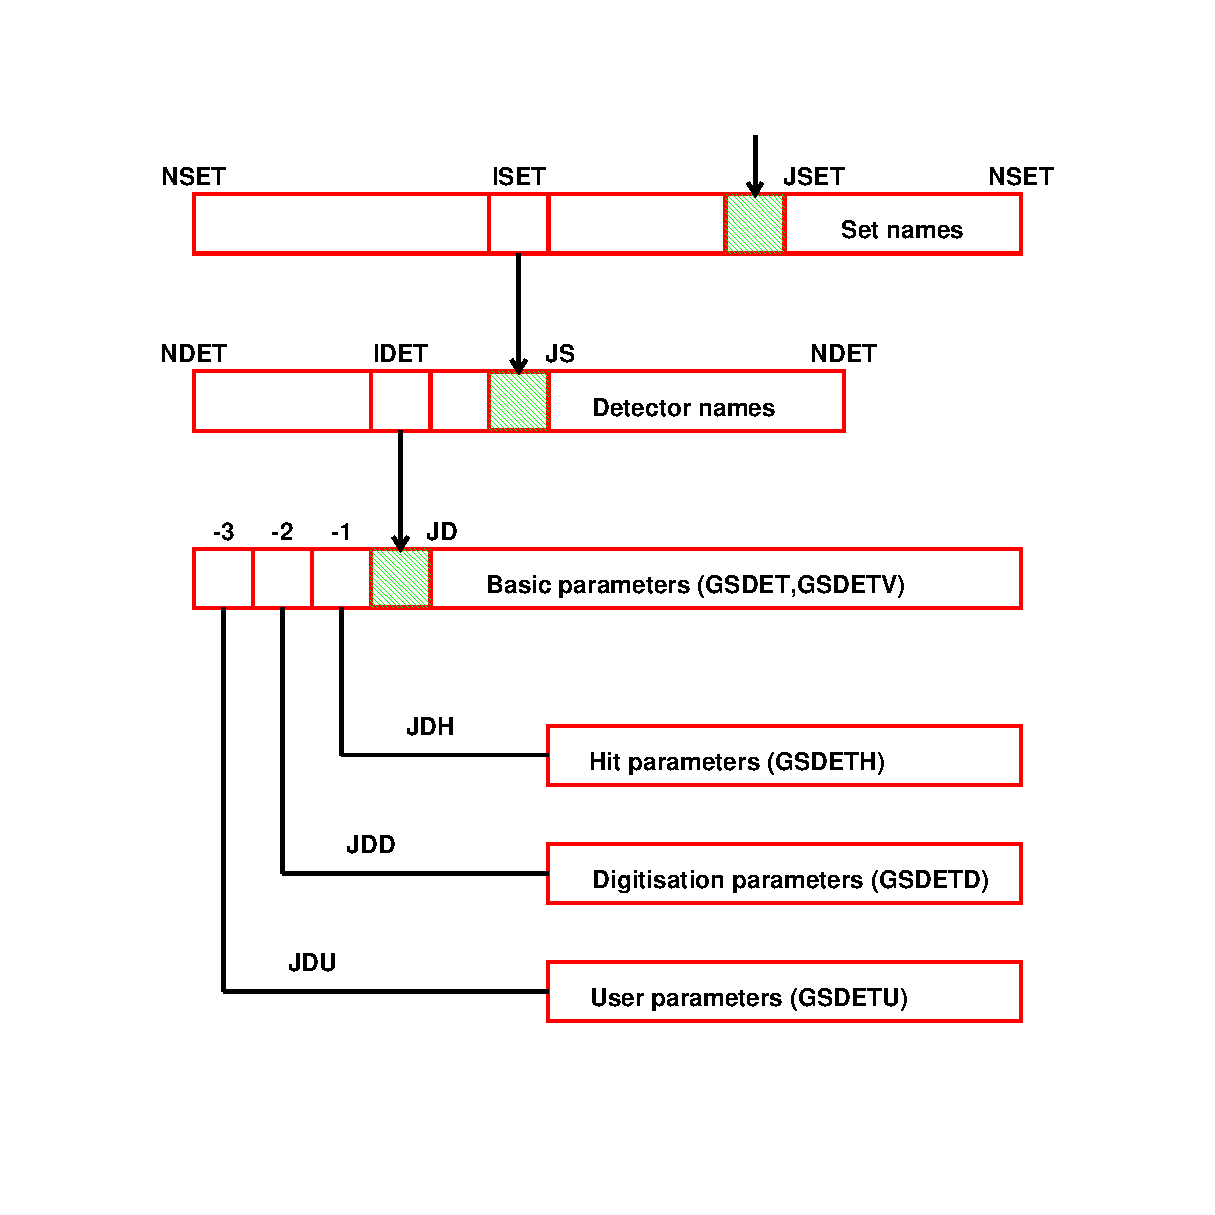
\epsfig{file=eps/hits199-1.eps,width=14cm}
     \caption{Example of geometrical tree structure}
     \label{fg:hits199-1}
\end{figure}
 
{\tt JS} = {\tt LQ(JSET-ISET)} pointer to detector set number {\tt ISET}
The {\tt JSET} data structure is filled by \Rind{GSDET}, 
\Rind{GSDETV}, \Rind{GSDETH}, \Rind{GSDETD}, \Rind{GSDETU} 
and possibly by \Rind{GSDETA}.
 

%%%%%%%%%%%%%%%%%%%%%%%%%%%%%%%%%%%%%%%%%%%%%%%%%%%%%%%%%%%%%%%%%%%
%                                                                 %
%  GEANT manual in LaTeX form                                     %
%                                                                 %
%  Michel Goossens (for translation into LaTeX)                   %
%  Version 1.00                                                   %
%  Last Mod. Jun  8 1993  1300   MG                               %
%                                                                 %
%%%%%%%%%%%%%%%%%%%%%%%%%%%%%%%%%%%%%%%%%%%%%%%%%%%%%%%%%%%%%%%%%%%
\Origin{R.Brun, F.Bruyant, W.Gebel, M.Maire}
\Submitted{01.11.83}                   \Revised{17.12.93}
\Version{Geant 3.16}                   \Routid{HITS200}

\Makehead{Routines to store and retrieve HITS}

\Shubr{GSAHIT}{(ISET,IDET,ITRA,NUMBV,HITS,IHIT*)}
\begin{DLtt}{MMMMMMMM}
\item[ISET]  ({\tt INTEGER}) set number (see below);
\item[IDET]  ({\tt INTEGER}) detector number;
\item[ITRA]  ({\tt INTEGER}) number of the track producing this hit
\item[NUMBV] ({\tt INTEGER}) array of volume numbers corresponding 
to list {\tt NAMESV} of {\tt GSDET};
\item[HITS] ({\tt REAL}) array of values for current hit elements;
\item[IHIT] ({\tt INTEGER}) current hit number, if 0 the
hit has not been stored.
\end{DLtt}

Stores element values for current hit into the data structure {\tt
JHITS}. The values {\tt ISET}, {\tt IDET} and {\tt NUMBV} can be found
in the corresponding variables of common \FCind{/GCSETS/}. These values
are set by the routine \Rind{GFINDS} every time that a particle is in
a defined detector.

\Shubr{GSCHIT}{(ISET,IDET,ITRA,NUMBV,HITS,NHSUM,IHIT*)}
Same action as \Rind{GSAHIT}, but in case the detector identified by
{\tt ISET}, {\tt IDET} and
{\tt NUMBV} contains already a hit for the same track, the routine will
make a cummulative sum for the latest {\tt NHSUM} elements of {\tt JHITS}.
The other previous elements of {\tt JHITS} are replaced.
That facility is particularly interesting in the case of
hits generated into a calorimeter. No packing (i.e. 32 bits per
hit element) should be requested for the
last {\tt NHSUM} hits in \Rind{GSDETH} and for these hits {\tt ORIG} should
be set to 0.

\Shubr{GPHITS}{(CHSET,CHDET)}
\begin{DLtt}{MMMMMMMM}
\item[CHSET] ({\tt CHARACTER*4}) set name,
if {\tt '*'} prints all {\tt JHITS} banks of all sets;
\item[CHDET] ({\tt CHARACTER*4}) detector name,
if {\tt '*'} prints hits in all detectors of set {\tt
CHSET}.
\end{DLtt}
Prints {\tt JHITS} banks for detector {\tt CHDET} of set {\tt CHSET}.
 
\Shubr{GFHITS}{(CHSET,CHDET,NVDIM,NHDIM,NHMAX,ITRS,NUMVS,
                ITRA*,NUMBV*,HITS*,NHITS*)}
 
\begin{DLtt}{MMMMMMMM}
\item[CHSET] ({\tt CHARACTER*4}) set name;
\item[CHDET] ({\tt CHARACTER*4}) detector name;
\item[NVDIM] ({\tt INTEGER}) 1$^{st}$ dimension of arrays {\tt NUMBV} and
{\tt NUMVS}: 1$\leq${\tt NVDIM}$\leq${\tt NV} argument of \Rind{GSDET};
\item[NHDIM] ({\tt INTEGER}) 1$^{st}$ dimension of array {\tt HITS}:
1$\leq${\tt NHDIM}$\leq${\tt NH} argument of \Rind{GSDETH};
\item[NHMAX] ({\tt INTEGER}) maximum number of hits to be returned, this 
should be not larger than the second dimension of array {\tt NUMBV} and
{\tt HITS};
\item[ITRS] ({\tt INTEGER}) number of the selected track,
if {\tt ITRS=0}, all tracks are taken;
\item[NUMVS] ({\tt INTEGER}) is a 1-dimension array of {\tt NVDIM}
elements that contains
the list of volume numbers which identify the selected detector,
0 is interpreted as 'all valid numbers';
\item[ITRA] ({\tt INTEGER}) is a 1-dim array of dimension {\tt NHMAX}
that contains on output
for each hit the number of the track which has produced it;
\item[NUMBV] ({\tt INTEGER}) 2-dim array ({\tt NVDIM,NHMAX})
that containis on output for each hit the
list of volume numbers which identify the detector, all values set to 
0 means that no more volumes are stored;
\item[HITS] ({\tt REAL}) 2-dim array ({\tt NHDIM,NHMAX}) that containis 
{\tt NHITS} hits;
\item[NHITS] ({\tt INTEGER}) number of hits returned, in case the total
number of hits is greater than {\tt NHMAX, NHITS} is set to
{\tt NHMAX+1} and {\tt NHMAX} hits are returned.
\end{DLtt}

This rotine returns the hits produced by track {\tt ITRS} (or by any track) in
the detector {\tt CHDET} identified by the list {\tt NUMVS}
belonging to set {\tt CHSET}.

\begin{DLtt}{MMMMMMMMMMMM}
\item[HITS(1,I)] is element 1 of hit number {\tt I};
\item[NUMBV(1,I)] is volume number 1 of hit number {\tt I};
\item[ITRA(I)] is the track number corresponding to hit number {\tt I};
\end{DLtt}

The arrays {\tt NUMVS, NUMBV, HITS}
and {\tt ITRA} must be dimensioned to:
\begin{verbatim}
    NUMVS(NVDIM)
    NUMBV(NVDIM,NHMAX)
    HITS(NHDIM,NHMAX)
    ITRA(NHMAX)
\end{verbatim}

\Shubr{GFPATH}{(ISET,IDET,NUMBV,NLEV*,LNAM*,LNUM*)}
\begin{DLtt}{MMMMMMMM}
\item[ISET] ({\tt INTEGER}) set number;
\item[IDET] ({\tt INTEGER}) detector number;
\item[NUMBV] ({\tt INTEGER}) array of numbers which identify uniquely
detector number {\tt IDET};
\item[NLEV] ({\tt INTEGER}) number of elements filled of arrays
{\tt LNAM} and {\tt LNUM};
\item[LNAM] ({\tt INTEGER}) array of {\tt NLEV} volume names stored in 
ASCII code in integers;
\item[LNUM] ({\tt INTEGER}) array of {\tt NLEV} copy numbers.
\end{DLtt}

This routine returns the list of volume names and numbers
which identify the complete ancestry in the {\tt JVOLUM} data structure of the
volume corresponding to the detector number {\tt IDET} in set
number {\tt ISET} and which is identified by the volume numbers {\tt NUMBV}
(see \Rind{GFHITS}).
 
\Rind{GFPATH} assumes that the detectors have been declared via 
\Rind{GSDETV} and not \Rind{GSDET}. The main use of \Rind{GFPATH} is to
prepare the lists {\tt LNAM} and {\tt LNUM} required  by the routine
\Rind{GLVOLU} to fill the common \FCind{/GCVOLU/}. Once \FCind{/GCVOLU/}
is properly filled, it is possible to use the {\tt GEANT} routines to
transform from the local to the master reference system and so on.
 

%%%%%%%%%%%%%%%%%%%%%%%%%%%%%%%%%%%%%%%%%%%%%%%%%%%%%%%%%%%%%%%%%%%
%                                                                 %
%  GEANT manual in LaTeX form                              %
%                                                                 %
%  Michel Goossens (for translation into LaTeX)                   %
%  Version 1.00                                                   %
%  Last Mod. Jan 24 1991  1300   MG + IB                          %
%                                                                 %
%%%%%%%%%%%%%%%%%%%%%%%%%%%%%%%%%%%%%%%%%%%%%%%%%%%%%%%%%%%%%%%%%%%
\Origin{R.Brun}
\Submitted{01.11.83}     \Revised{18.12.93}
\Version{Geant 3.16}     \Routid{HITS299}
\Makehead{The JHITS data structure}

\begin{figure}[hbt]
     \centering
     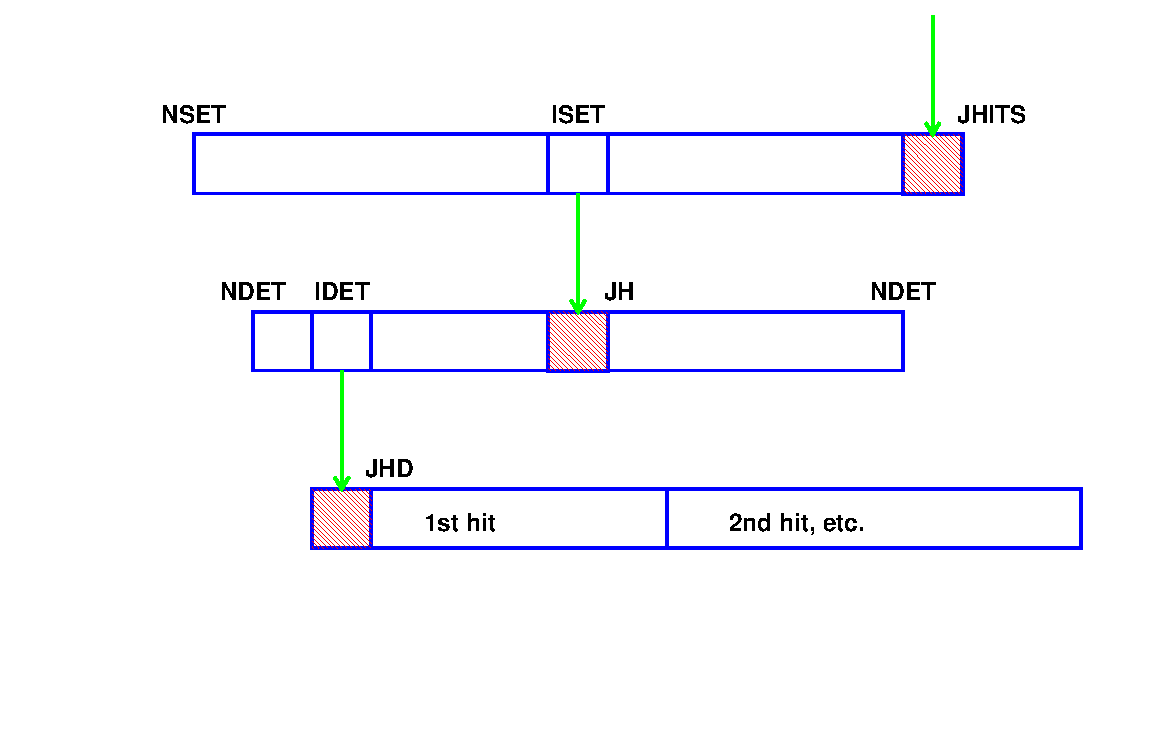
\epsfig{file=eps/hits299-1.eps,width=14cm}
     \caption{Layout of the {\tt JHITS} data structure}
     \label{fg:hits299-1}
\end{figure}

\begin{tabular}{lp{12cm}}
\tt JH=LQ(JHITS-ISET) & pointer to hits structure for set number {\tt ISET} \\
\tt IQ(JH+IDET) & number of words used for storing the hits
of detector number {\tt IDET} \\
\tt JHD=LQ(JH-IDET) & pointer to hits bank for detector number {\tt IDET} of
set number {\tt ISET} \\
\tt IQ(JHD+1) & 1$^{st}$ word of 1$^{st}$ hit \\
\tt IQ(JHD+NWH+1) & 1$^{st}$ word of 2$^{nd}$ hit \\
\tt JS=LQ(JSET-ISET) & pointer to the structure containing the description
of set number {\tt ISET} \\
\tt JD=LQ(JS-IDET) & pointer to the bank containing the description of detector
number {\tt IDET} of set number {\tt ISET} \\
\tt NWH=IQ(JD+3) & number of words in which a hit of detector
number {\tt IDET} of set number {\tt ISET} is stored
\end{tabular}

The {\tt JHITS} structure is filled with the routines \Rind{GSAHIT} and
\Rind{GSCHIT}.
The routine \Rind{GFHITS} can be used to get the hits for a detector
{\tt IDET} in set {\tt ISET}.

%%%%%%%%%%%%%%%%%%%%%%%%%%%%%%%%%%%%%%%%%%%%%%%%%%%%%%%%%%%%%%%%%%%
%                                                                 %
%  GEANT manual in LaTeX form                                     %
%                                                                 %
%  Version 1.00                                                   %
%                                                                 %
%  Last Mod.  9 Jun 1993  1300   MG                               %
%                                                                 %
%%%%%%%%%%%%%%%%%%%%%%%%%%%%%%%%%%%%%%%%%%%%%%%%%%%%%%%%%%%%%%%%%%%
\Origin{R.Brun, W.Gebel}
\Submitted{10.08.84}       \Revised{18.12.93}
\Version{Geant 3.16}       \Routid{HITS300}

\Makehead{Routines to store and retrieve DIGItisations}

\Shubr{GSDIGI}{(ISET,IDET,LTRA,NTRA,NUMBV,KDIGI,IDIG*)}
\begin{DLtt}{MMMMMMMM}
\item[ISET] ({\tt INTEGER}) set number;
\item[IDET] ({\tt INTEGER}) detector number;
\item[LTRA] ({\tt INTEGER}) array of {\tt NTRA} track numbers producing 
this digitisation;
\item[NUMBV] ({\tt INTEGER}) volume numbers corresponding to list {\tt NAMESV} 
of \Rind{GSDET};
\item[KDIGI] ({\tt INTEGER}) array of current digisation elements;
\item[IDIG] ({\tt INTEGER}) stored digitisation number, if 0, digitisation 
has not been stored.
\end{DLtt}
Stores element values for current digitisation
into the data structure {\tt JDIGI}.

\Shubr{GPDIGI}{(CHSET,CHDET)}
\begin{DLtt}{MMMMMMMM}
\item[CHSET] ({\tt CHARACTER*4}) set name,
if {\tt '*'} prints all {\tt JDIGI} banks of all sets;
\item[CHDET] ({\tt CHARACTER*4}) detector name, if {\tt '*'} prints 
digitisations in all detectors of set;
{\tt CHSET}
\end{DLtt}
Prints {\tt JDIGI} banks for detector {\tt CHDET} of set {\tt CHSET}.
 
\Shubr{GFDIGI}{(CHSET,CHDET,NTDIM,NVDIM,NDDIM,NDMAX,NUMVS,
                LTRA*,NTRA*,NUMBV*,KDIGI*,NDIGI*)}
\begin{DLtt}{MMMMMMMM}
\item[CHSET] ({\tt INTEGER}) set name;
\item[CHDET] ({\tt INTEGER}) detector name;
\item[NTDIM] ({\tt INTEGER}) 1$^st$ dimension of {\tt LTRA}, maxmum number of 
tracks contributing to each hit to be returned;
\item[NVDIM] ({\tt INTEGER}) 1$^{st}$ dimension of arrays {\tt NUMVS}, 
{\tt NUMBV}, same as argument {\tt NV} of \Rind{GSDET};
\item[NDDIM] ({\tt INTEGER}) 1$^{st}$ dimension of {\tt KDIGI}, same
as argument {\tt ND} of \Rind{GSDETD};
\item[NDMAX] ({\tt INTEGER}) maximum number of digitisations to be returned,
second dimension of arrays {\tt NTDIM}, {\tt NUMBV} and {\tt KDIGI};
\item[NUMVS] ({\tt INTEGER}) is a 1-dim array of length {\tt NVDIM}
that contains the copy numbers identifying the detector to be selected, all 
0 is interpreted as all copies of detector {\tt CHDET};
\item[LTRA] ({\tt INTEGER}) is a 2-dim array {\tt NTDIM,NDMAX} that contains
for each digitisation the numbers of the tracks which have produced it;
\item[NTRA] ({\tt INTEGER}) is a 1-dim array of length {\tt NDMAX} that contains,
for each digitisation, the number of tracks contributing,
in case this number is greater than {\tt NTDIM}, only the first
{\tt NTDIM} corresponding tracks are returned on {\tt LTRA};
\item[NUMBV] ({\tt INTEGER}) is a 2-dim array {\tt NVDIM,NDMAX} that contains,
for each digitisation, the
list of volume numbers which identify each detector;
\item[KDIGI] ({\tt INTEGER}) is a 2-Dim array {\tt NDDIM,NDMAX} that contains 
the {\tt NDIGI} digitisations returned;
\item[NDIGI] ({\tt INTEGER}) is the total number of digitisations in this 
detector,
in case the total number of digitisations is greater than {\tt NDMAX},
{\tt NDIGI} is set to {\tt NDMAX+1} and only {\tt NDMAX} digitisations are
returned.
\end{DLtt}
Returns the digitisations for the detector {\tt CHDET} identified by the list 
of copy numbers {\tt NUMVS} belonging to set {\tt CHSET}. The maning of
the variables is the following:

\begin{tabular}{lp{10cm}}
\tt KDIGI(1,I) & digitisation element 1 for digitisation number {\tt I} \\
\tt NUMBV(1,I) & first volume number for digitisation number {\tt I} \\
\tt LTRA (1,I) & number of the first track contributing to digitisation 
number {\tt I} \\
\end{tabular}

In the calling routine, the arrays {\tt LTRA, NTRA, NUMVS, NUMBV,
KDIGI} must be dimensioned to:
\begin{verbatim}
      LTRA (NTDIM,NDMAX)
      NTRA (NDMAX)
      NUMVS(NVDIM)
      NUMBV(NVDIM,NDMAX)
      KDIGI(NDDIM,NDMAX)
\end{verbatim}
 

%%%%%%%%%%%%%%%%%%%%%%%%%%%%%%%%%%%%%%%%%%%%%%%%%%%%%%%%%%%%%%%%%%%
%                                                                 %
%  GEANT manual in LaTeX form                              %
%                                                                 %
%  Michel Goossens (for translation into LaTeX)                   %
%  Version 1.00                                                   %
%  Last Mod. Jan 24 1991  1300   MG + IB                          %
%                                                                 %
%%%%%%%%%%%%%%%%%%%%%%%%%%%%%%%%%%%%%%%%%%%%%%%%%%%%%%%%%%%%%%%%%%%
\Origin{R.Brun}
\Submitted{01.11.83}     \Revised{18.12.93}
\Version{Geant 3.16}     \Routid{HITS399}
\Makehead{The JDIGI data structure}

\begin{figure}[hbt]
     \centering
     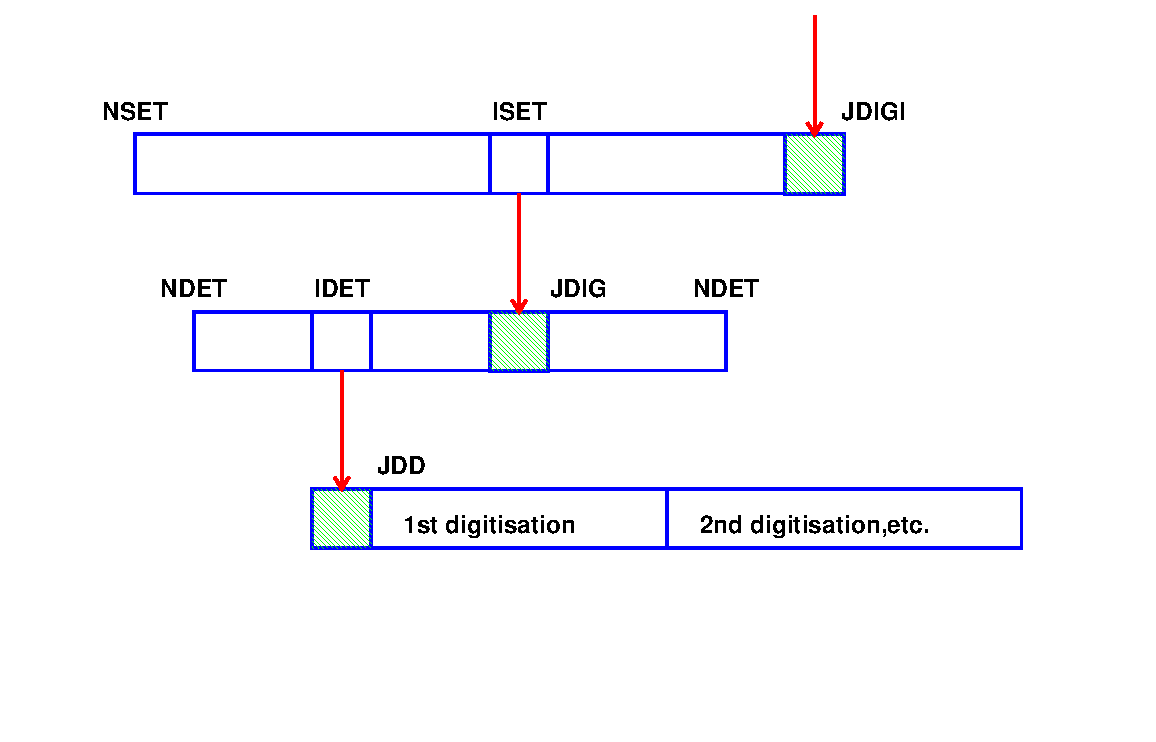
\epsfig{file=eps/hits399-1.eps,width=14cm}
     \caption{Layout of the {\tt JDIGI} data structure}
     \label{fg:hits399-1}
\end{figure}

\begin{tabular}{lp{10cm}}
\tt JDIG=LQ(JDIGI-ISET) & pointer to digitisations structure for set 
number {\tt ISET}\\
\tt JDD=LQ(JDIG-IDET) & pointer to digitisations of detector number
{\tt IDET} of set number {\tt ISET} \\
\tt IQ(JDIG+IDET) & pointer to last word of last digitisation for detector
number {\tt IDET} \\
\tt IQ(JDD+1) & 1$^{st}$ word of 1$^{st}$ digitisation \\
\tt IQ(JDD+N+1) & 1$^{st}$ word of 2$^{nd}$ digitisation\\
\tt JS=LQ(JSET-ISET) & pointer to the structure containing the description
of digitisations of set number {\tt ISET} \\
\tt JD=LQ(JS-IDET) & pointer to the structure containing the description
of digitisations of detector number {\tt IDET} \\
\tt NWD=IQ(JD+5) & number of elements of digitisation of set/detector
{\tt ISET}/{\tt IDET}  \\
\tt NTRA & number of tracks contributing to digitisation\\
\tt N=NWD+NTRA/2+1 & N varies from digitisation to digitisation 
\end{tabular}

The {\tt JDIGI} structure is filled with the routine \Rind{GSDIGI}.
The routine \Rind{GFDIGI} can be used to get the digitisations for
a detector {\tt IDET} in set {\tt ISET}.
 

%%%%%%%%%%%%%%%%%%%%%%%%%%%%%%%%%%%%%%%%%%%%%%%%%%%%%%%%%%%%%%%%%%%
%                                                                 %
%  GEANT manual in LaTeX form                                     %
%                                                                 %
%  Michel Goossens (for translation into LaTeX)                   %
%  Version 1.00                                                   %
%  Last Mod. Jan 24 1991  1300   MG + IB                          %
%                                                                 %
%%%%%%%%%%%%%%%%%%%%%%%%%%%%%%%%%%%%%%%%%%%%%%%%%%%%%%%%%%%%%%%%%%%
\Origin{R.Brun,H. Boerner}
\Submitted{01.10.81}   \Revised{18.12.93}
\Version{Geant 3.10}   \Routid{HITS400}

\Makehead{Intersection of a track with a cylinder or a plane}

\Shubr{GICYL}{(R,X1,X2,S1,S2,IC,XINT*,SINT*,PZINT*,IFLAG*)}
\begin{DLtt}{MMMMMMMM}
\item[R] ({\tt REAL}) radius of cylinder in cm;
\item[X1] ({\tt REAL}) array of 6, ($x$, $y$, $z$, $dx/ds$, 
$dy/ds$, $dz/ds$) of 1$^{st}$ point;
\item[X2] ({\tt REAL}) array of 6, ($x$, $y$, $z$, $dx/ds$, 
$dy/ds$, $dz/ds$) of 2$^{nd}$ point;
\item[S1] ({\tt REAL}) track length $s$ at 1$^{st}$ point;
\item[S2] ({\tt REAL}) track length $s$ at 2$^{nd}$ point;
\item[IC] ({\tt INTEGER}) type of interpolation:
\begin{DLtt}{MMMM}
\item[1] straight line defined as ({\tt Xi(1),Xi(2),Xi(3)}) + $s$
({\tt Xi(4),Xi(5),Xi(6)}), where {\tt i} is {\tt 1} or {\tt 2} according
to which of the two points is {\it inside} the cylinder;
\item[2] straight line going from ({\tt X1(1),X1(2),X1(3)}) to
({\tt X2(1),X2(2),X2(3)});
\item[3] third degree curve with:
\[
\vec{P}(s)  =  \vec{a} \; s^3 + \vec{b} \; s^2 +\vec{c} \; s +\vec{d} 
\hspace{1.2cm}
\mbox{\tt X}i   =  \left ( \vec{P}(\mbox{\tt S}i), \; 
\left . \frac{d\vec{P}}{ds} \right |_{s=\mbox{\tt S}i} \right ) \hspace{5mm}
i=1,2
\]
\end{DLtt}
\item[XINT] ({\tt REAL}) array of 6 $x$, $y$, $z$, $dx/ds$, $dy/ds$, $dz/ds$ 
at intersection point;
\item[SINT] ({\tt REAL}) {\tt S} at intersection point;
\item[PZINT] ({\tt REAL}) $\phi$, $z$, $d\phi/dr$, $dz/dr$ in
cylindrical coordinates at intersection point;
\item[IFLAG] ({\tt INTEGER}) return flag:
\begin{DLtt}{MMMM}
\item[0] track does not intersect cylinder;
\item[1] track intersects cylinder.
\end{DLtt}
\end{DLtt}
Calculates intersection of track with a cylinder
of radius {\tt R}. The track is approximated by a cubic
in the track length. To improve stability, the coordinate system
is shifted.

\Shubr{GIPLAN}{(YC,X1,X2,S1,S2,IC,XINT*,SINT*,PZINT*,IFLAG*)}
The arguments have the same meaning than in the previous routine, apart from:
\begin{DLtt}{MMMMMMMM}
\item[YC] ({\tt REAL}) $y$ coordinate of plane;
\end{DLtt}
Calculates intersection of track with a plane parallel to $x-z$.
The track is approximated by a cubic
in the track length. To improve stability, the coordinate system
is shifted.

{\bf Note}: the default accuracy is 10 microns. The value
of {\tt EPSI} (internal variable) must be changed for a better precision.

%%%%%%%%%%%%%%%%%%%%%%%%%%%%%%%%%%%%%%%%%%%%%%%%%%%%%%%%%%%%%%%%%%%
%                                                                 %
%  GEANT manual in LaTeX form                                     %
%                                                                 %
%  Michel Goossens (for translation into LaTeX)                   %
%  Version 1.00                                                   %
%  Last Mod. Jan 24 1991  1300   MG + IB                          %
%                                                                 %
%%%%%%%%%%%%%%%%%%%%%%%%%%%%%%%%%%%%%%%%%%%%%%%%%%%%%%%%%%%%%%%%%%%
\Origin{GEANT2}
\Submitted{01.10.81}   \Revised{19.12.93}
\Version{Geant 3.16}\Routid{HITS500}
\Makehead{Digitisation for drift- or MWP- Chambers}

\Shubr{GPDRIF}{(DETREP,HITREP,IOUT*)}
\begin{DLtt}{MMMMMMMM}
\item[DETREP] ({\tt REAL}) array of 6 with detector description:
\begin{DLtt}{MMMM}
\item[1] number of wires;
\item[2] wire spacing in cm;
\item[3] $\sin(\alpha)$;
\item[4] $\cos(\alpha)$;
\item[5] distance of wire 1 from the origin in cm;
\item[6] drift velocity (cm/nsec)
\end{DLtt}
\item[HITREP] ({\tt REAL}) array of 2 with track description:
\begin{DLtt}{MMMM}
\item[1] $x$ coordinate of intersection;
\item[2] $y$ coordinate of intersection;
\end{DLtt}
\item[IOUT] ({\tt INTEGER}) result of digitisation:
\begin{DLtt}{MMMM}
\item[1] wire number;
\item[2] drift time (signed to avoid left/right ambiguity).
\end{DLtt}
\end{DLtt}
Digitisation routine for a plane drift chamber. The drift chamber is supposed
to be in the $x-y$ plane. The normal to the wires in the $x-y$ plane and the
$z$ axis form an angle $\alpha$.

\Shubr{GCMWPC}{(DETREP,HITREP,IOUT*)}
\begin{DLtt}{MMMMMMMM}
\item[DETREP] ({\tt REAL}) array of 6 with detector description:
\begin{DLtt}{MMMM}
\item[1] number of wires;
\item[2] wire spacing (radians);
\item[3] $d\theta/dz$ along the wires;
\item[4] $\theta$ of a point on wire 1;
\item[5] $z$ of a point on wire 1 corresponding to $\theta$={\tt DETREP(4)};
\item[6] gap width;
\end{DLtt}
\item[HITREP] ({\tt REAL}) array of 4 with track description:
\begin{DLtt}{MMMM}
\item[1] $\theta$ coordinate of intersection;
\item[2] $z$ coordinate;
\item[3] $d\theta/dr$;
\item[4] $dz/dr$;
\end{DLtt}
\item[IOUT] ({\tt INTEGER}) array of 4 with result of digitisation:
\begin{DLtt}{MMMM}
\item[1] wire number (-1 if missing);
\item[2] cluster size;
\item[3] wire number of second cluster if any;
\item[4] cluster size;
\end{DLtt}
\end{DLtt}
Routine to compute one or two digitisations produced
by a hit on a cylindrical {\tt MWPC}. The chamber is a cylinder of thickness
{\tt DETREP(6)} which should be small compared with the radius.

\Shubr{GPMWPC}{(DETREP,HITREP,IOUT*)}
\begin{DLtt}{MMMMMMMM}
\item[DETREP] ({\tt REAL}) array of 6 with detector description:
\begin{DLtt}{MMMM}
\item[1] number of wires;
\item[2] wire spacing (radians);
\item[3] $\sin(\alpha)$;
\item[4] $\cos(\alpha)$;
\item[5] distance of wire 1 from the origin in cm;
\item[6] gap width;
\end{DLtt}
\item[HITREP] ({\tt REAL}) array of 4 with track description:
\begin{DLtt}{MMMM}
\item[1] $x$ coordinate of intersection;
\item[2] $y$ coordinate of intersection;
\item[3] $dx/dz$;
\item[4] $dy/dz$;
\end{DLtt}
\item[IOUT] ({\tt INTEGER}) array of 2 with result of digitisation:
\begin{DLtt}{MMMM}
\item[1] wire number (-1 if missing);
\item[2] cluster size;
\end{DLtt}
\end{DLtt}
Digitisation routine for a plane {\tt MWPC}.
 

%%%%%%%%%%%%%%%%%%%%%%%%%%%%%%%%%%%%%%%%%%%%%%%%%%%%%%%%%%%%%%%%%%%
%                                                                 %
%  GEANT manual in LaTeX form                              %
%                                                                 %
%  Michel Goossens (for translation into LaTeX)                   %
%  Version 1.00                                                   %
%  Last Mod. Jan 24 1991  1300   MG + IB                          %
%                                                                 %
%%%%%%%%%%%%%%%%%%%%%%%%%%%%%%%%%%%%%%%%%%%%%%%%%%%%%%%%%%%%%%%%%%%
\Origin{W.Mitaroff}
\Submitted{21.02.85}               \Revised{19.12.93}
\Version{Geant 3.16}               \Routid{HITS510}

\Makehead{Digitisation for drift chambers}

\Shubr{GCDRIF}{(RADD,ZMIN,ZMAX,DETREP,HITREP,IOUT*)}
\begin{DLtt}{MMMMMMMM}
\item[RADD] ({\tt REAL}) radius of cylindrical chamber in cm;
\item[ZMIN] ({\tt REAL}) $z$ of lower end of cylindrical chamber;
\item[ZMAX] ({\tt REAL}) $z$ of upper end of cylindrical chamber;
\item[DETREP] ({\tt REAL}) array of 8 with detector description:
\begin{DLtt}{MMMM}
\item[1] number of wires;
\item[2] wire spacing in $\phi$ (radians);
\item[3] cosine of wire angle with respect to the $z$ axis;
\item[4] sine of wire angle  with respect to the $z$ axis 
(signed like $d\phi/dz$);
\item[5] $d\phi/dz$ along wire;
\item[6] $\phi$ of point with $z=0$ on wire 1;
\item[7] drift velocity (cm nsec$^{-1}$);
\item[8] if $>0$ user routine \Rind{GUDTIM}
will be called to calculate drift time;
\end{DLtt}
\item[HITREP] ({\tt REAL}) array of 4 describing the track:
\begin{DLtt}{MMMM}
\item[1] $\phi$ coordinate of intersection;
\item[2] $z$ coordinate of intersection;
\item[3] $d\phi/dr$;
\item[4] $dz/dr$;
\end{DLtt}
\item[IOUT] ({\tt INTEGER}) array of 4 with digitisation information:
\begin{DLtt}{MMMM}
\item[1] wire number (1...{\tt NWI} with increasing phi), -1 if {\tt DETREP}
parameters are inconsistent;
\item[2] drift time in nsec, $>0$ if $\phi(hit)>\phi(wire)$;
\item[3] digitised current division information
(relative position of charge along wire, per mille);
\item[4] amount of charge deposited onto wire.
\end{DLtt}
\end{DLtt}
Digitisation routine for a cylindrical drift chamber.
 
\begin{figure}[hbt]
     \centering
%    \epsfig{file=eps/hits510-1.eps,width=14cm}
\begin{verbatim}
                        Charge                     
         .              |                        .
         |              .                        |
         =========================================  SENSE WIRE
     ...................................................> Z (cm)
         Z              Z                        Z 
          l                                       u
     ...............................................> ICD (0<ICD<1000)
         0              ICD                      1000
               ICD                (1000-ICD)
\end{verbatim}
     \caption{Coordinate system along the wire}
     \label{fg:hits510-1}
\end{figure}

Knowing the position $Z$ of the deposit of charge we can calculate
\[
\mbox{\tt ICD} = L \frac{Z-Z_l}{Z_u -Z_l} 
\]
where $L=1000$ in the
program. This is the information stored into {\tt IOUT(3)}.

\Shubr{GCDERR}{(ICD*,ERP,ERS)}
\begin{DLtt}{MMMMMMMM}
\item[ICD] ({\tt INTEGER}) digitised current division information 
($\leq\mbox{\tt ICD}\leq1000$), overwritten on output with the
modified value taking into account the errors;
\item[ERP] ({\tt REAL}) variance of Gaussian pedestal errors 
on the measured
pulse heights relative to the sum of the pulse heights;
\item[ERS] ({\tt REAL}) variance of Gaussian slope 
errors on the measured
pulse heights relative to the each pulse heights.
\end{DLtt}
Routine to calculate the error on the current division
information as obtained by \Rind{GCDRIF}.
Here we assume that {\tt ICD} has been determined by measuring the pulse heights 
$I_1, I_2$ at the two ends of the wire with the formula:
\[
\mbox{\tt ICD} = L \; \frac{I_2}{I_+} 
\mbox{\hspace{1cm}with\hspace{1cm}}  I_+ = I_1+I_2 
\]
Its error is determined by:
\[
\delta \mbox{\tt ICD} = - \frac{\mbox{\tt ICD}}{I_+} \delta I_1 + 
\frac{L-\mbox{\tt ICD}}{I_+}  \delta I_2
\mbox{\hspace{5mm}and\hspace{5mm}}
\delta I_1 = \delta_1 + \epsilon_1 \; I_1  \mbox{\hspace{3mm};\hspace{3mm}}
\delta I_2 = \delta_2 + \epsilon_2 \; I_2 
\]
 
 
$\delta_1$ and $\delta_2 $ are of dimension {\tt [I]} and represent the 
{\it pedestal} errors. $\epsilon_1$ and $\epsilon_2$ are the {\it slope} errors.
Errors are independent (no correlations), with a Gaussian distribution with 
average 0 and {\tt ERP} as relative variance for pedestals $\delta_i/I_+$ 
and {\tt ERS} as variance for slopes $\epsilon_i$.  This gives the final result
 
\[
\delta \mbox{\tt ICD}   = \underbrace{-\frac{\delta_1}{I_+}\mbox{\tt ICD} +
                 \frac{\delta_2}{I_+}(L-\mbox{\tt ICD})}_{\mbox{\it pedestals}}
               +
 \underbrace{(\epsilon_2-\epsilon_1)
\frac{\mbox{\tt ICD}(L-\mbox{\tt ICD})}{L}}_{\mbox{\it slope}}
\]

\Rind{GCDERR} sets the {\tt ICD} obtained from \Rind{GCDRIF} to
$\mbox{\tt ICD}=\mbox{\tt ICD}+\delta \mbox{\tt ICD}$ with 
$ 0 \leq \mbox{\tt ICD}\leq L$.

\Sfunc{GUDTIM}{VALUE = GUDTIM(DETREP,HITREP,IW1,DIS)}
The arguments have the same meaning than for \Rind{GCDRIF} apart from:
\begin{DLtt}{MMMMMMMM}
\item[IW1] ({\tt INTEGER}) wire number which will generate a signal;
\item[DIS] ({\tt REAL}) distance from the track to the wire;
\end{DLtt}
This function has to be written by the user to return the drift time
in nanoseconds.

\putbib[cnasbibl,geabibl]
\end{bibunit}

%  ==================== Index material ============================

\setcounter{page}{1}%                                Reset page counter
\def\Rtnr{Index}%Dummy routine name to appear at bottom of page
\input{\jobname.ind} % index

\end{document}
